\documentclass[11pt]{scrreprt}
\usepackage[sexy,bib,noasy]{evan}
\input{preamble.sty}
\addbibresource{references.bib}

\begin{document}
\title{CSE402: Optimisation}
\author{Irfan Rahman \&\\ Mahmudul Hasan Turjoy}
\date{Last updated: \today}
\maketitle

\begin{abstract}
	These notes were taken in the course \textbf{CSE402: Optimisation} taught at BRAC University in Fall 2026 by Nafis Faisal. The main text used is \cite{algoForOp}. All errors are our responsibilty. If you find any error, please email us at \href{mailto:mh.turjoy@yahoo.com}{mh.turjoy@yahoo.com} or \href{mailto:rasib.rahman.04@gmail.com}{rasib.rahman.04@gmail.com}, even if it is something very small, even if you're not sure. Some of the content in these notes, mostly the tedious parts like bookish definitions, examples, figures, and other repetitive or straightforward sections, has been written with the help of Generative AI.
\end{abstract}

\tableofcontents

\lecture_date{06/10/2026}
\chapter{Lecture 01}

Mathematical language of this course is linear algebra (of real vector spaces) and multivariable calculus. In this lecture, we will give a brief review of linear algebra.

\section{Review on linear algebra}

\textbf{Notation.} Let \( a_1, a_2, \ldots, a_n \) be a finite sequence of real numbers. We will denote the sum

\begin{equation}
	S = a_1 + a_2 + \cdots + a_n
	\label{eq:lecture-01-1}
\end{equation}

by

\begin{equation}
	S = \sum_{k=1}^{n} a_k.
	\label{eq:lecture-01-2}
\end{equation}

We have the following useful identities:

\begin{equation}
	\sum_{k=1}^{n} k = \frac{n(n+1)}{2},
	\label{eq:lecture-01-3}
\end{equation}

\begin{equation}
	\sum_{k=1}^{n} k^2 = \frac{n(n+1)(2n+1)}{6}.
	\label{eq:lecture-01-4}
\end{equation}

\subsection{Vectors}
\begin{definition}[\( \mathbb{R} \)-vector space]
	Let $V$ be a non-empty set. The set $V$ equipped with two binary operations
	\[
		+: V \times V \rightarrow V
	\]

	called \textit{vector addition}, and

	\[
		\cdot : \mathbb{R} \times V \rightarrow V
	\]

	called \textit{scalar multiplication} is called a \textbf{vector space over \( \mathbb{R} \)} or \( \mathbb{R} \)-\textbf{vector space} if for all $u,v,w \in V$ and all $a,b \in \mathbb{F}$, the following axioms hold:

	\begin{enumerate}
		\item \textbf{Closure under addition:}
		      \begin{equation}
			      u+v \in V
			      \label{eq:r-vector-space-1}
		      \end{equation}

		\item \textbf{Commutativity of addition:}
		      \begin{equation}
			      u+v=v+u
			      \label{eq:r-vector-space-2}
		      \end{equation}

		\item \textbf{Associativity of addition:}
		      \begin{equation}
			      (u+v)+w=u+(v+w)
			      \label{eq:r-vector-space-3}
		      \end{equation}

		\item \textbf{Existence of zero vector:}
		      There exists a vector $0 \in V$ such that
		      \begin{equation}
			      u+0=u
			      \label{eq:r-vector-space-4}
		      \end{equation}

		\item \textbf{Existence of additive inverse:}
		      For every $u\in V$, there exists $-u\in V$ such that
		      \begin{equation}
			      u+(-u)=0
			      \label{eq:r-vector-space-5}
		      \end{equation}

		\item \textbf{Closure under scalar multiplication:}
		      \begin{equation}
			      au\in V
			      \label{eq:r-vector-space-6}
		      \end{equation}

		\item \textbf{Distributivity of scalar multiplication over vector addition:}
		      \begin{equation}
			      a(u+v)=au+av
			      \label{eq:r-vector-space-7}
		      \end{equation}

		\item \textbf{Distributivity of scalar multiplication over field addition:}
		      \begin{equation}
			      (a+b)u=au+bu
			      \label{eq:r-vector-space-8}
		      \end{equation}

		\item \textbf{Associativity of scalar multiplication:}
		      \begin{equation}
			      a(bu)=(ab)u
			      \label{eq:r-vector-space-9}
		      \end{equation}

		\item \textbf{Identity element of scalar multiplication:}
		      \begin{equation}
			      1u=u
			      \label{eq:r-vector-space-10}
		      \end{equation}

	\end{enumerate}

	Hence, $(V,+,\cdot)$ is called a vector space over the field $\mathbb{R}$. Elements of \( V \) are called \textbf{vectors} and elements of \( \mathbb{R} \) are called \textbf{scalars}.
\end{definition}

\textbf{Convention.} From now on, vector space means \( \mathbb{R} \)-vector space, unless stated otherwise.

In this course, we will work with only the following special example of \( \mathbb{R} \)-vector space.
\begin{example}
	Let
	\begin{equation}
		V \coloneq \mathbb{R}^n = \{ [x_1, x_2 \ldots, x_n]^T \mid x_1, x_2, \ldots, x_n \in \mathbb{R} \}.
		\label{eq:vectors-1}
	\end{equation}

	For \( [x_1, x_2 \ldots, x_n]^T, [y_1, y_2 \ldots, y_n]^T \in V  \) and \( \alpha \in \mathbb{R} \) define addition (\( + \)) and scalar multiplication (\( \cdot \)), respectively as follows:

	\begin{equation}
		\begin{bmatrix} x_1\\ x_2\\ \vdots\\ x_n \end{bmatrix} + \begin{bmatrix} y_1\\ y_2\\ \vdots\\ y_n \end{bmatrix} = \begin{bmatrix} x_1 + y_1\\ x_2 + y_2\\ \vdots\\ x_n + y_n \end{bmatrix},
		\label{eq:vectors-2}
	\end{equation}

	\begin{equation}
		\alpha \cdot \begin{bmatrix} x_1\\ x_2\\ \vdots\\ x_n \end{bmatrix} = \begin{bmatrix} \alpha x_1\\ \alpha x_2\\ \vdots\\ \alpha x_n \end{bmatrix}.
		\label{eq:vectors-3}
	\end{equation}

	Then it is an easy check that \( V = \mathbb{R}^n \) forms an \( \mathbb{R} \)-vector space.
\end{example}

\subsection{Linear transformations}
In this course, we are mostly\todo{Not sure about that} concerned with following special functions between vector spaces:

\begin{definition}[Linear transformation]
	Let \( V, W \) be two vector space. A \textbf{linear transformation} from \( V \) to \( W \) is a function \( T: V \to W \) such that for all \( \mathbf{x}, \mathbf{y} \in V \) and \( \alpha \in \mathbb{R} \) the following holds true:
	\begin{itemize}
		\item \textbf{Additivity.}
		      \begin{equation}
			      T(\mathbf{x} + \mathbf{y}) = T(\mathbf{x}) + T(\mathbf{y}).
			      \label{eq:linear-transformation-1}
		      \end{equation}

		\item \textbf{Homogeneity.}
		      \begin{equation}
			      T(\alpha \cdot \mathbf{x}) = \alpha \cdot T(\mathbf{x}).
			      \label{eq:linear-transformation-2}
		      \end{equation}
	\end{itemize}
\end{definition}

\todo{Need to add visualisation of additivity and homogeneity property of a linear transformation.}

\begin{example}
	Let \( V \coloneq \mathbb{R}^n, W \coloneq \mathbb{R}^m \). An \( m \times n \) matrix \( M \) then defines a linear transformation \( M : \mathbb{R}^n \to \mathbb{R}^m\)\footnote{Here, we are denoting the linear transformation determined by the matrix \( M \) by the same letter \( M \) using abuse of notation.} as follows:

	For \( \mathbf{x} \in \mathbb{R}^n \),

	\begin{equation}
		M(\mathbf{x}) \coloneq M \mathbf{x}.
		\label{eq:linear-transformations-1}
	\end{equation}

	Here, \( M \) is an \( m \times n \) matrix, \( \mathbf{x} \) can is an \( n \times 1 \) matrix. So \( M \mathbf{x} \) is an \( m \times 1 \) matrix. Therefore, \( M \) is indeed a function from \( \mathbb{R}^n \) to \( \mathbb{R}^m \).

	Furthermore, for all \( \mathbf{x}, \mathbf{y} \in \mathbb{R}^n \) and \( \alpha \in \mathbb{R} \), the following holds by the properties of matrix multiplication:

	\begin{equation}
		M(\mathbf{x} + \mathbf{y}) = M \mathbf{x} + M \mathbf{y},
		\label{eq:linear-transformations-2}
	\end{equation}

	\begin{equation}
		M(\alpha \mathbf{x}) = \alpha M \mathbf{x}
		\label{eq:linear-transformations-3}
	\end{equation}

	Hence, \( M \) is indeed a linear transformation.

\end{example}

Surprising fact is that an arbitrary linear transformation also comes from a matrix. Before that, we need the idea of basis.

\subsection[Basis and dimension of Rn]{Basis and dimension of \(\mathbb{R}^n\)}

Consider the vector space

\begin{equation}
	\mathbb{R}^2= \left\{[x, y]^T:x,y\in\mathbb{R}\right\}.
	\label{eq:basis-and-dimension-of-r-1}
\end{equation}

A natural question is: how many vectors are required to generate every vector in
\(\mathbb{R}^2\)? Answer to this question is particularly useful in the context
of linear transformations.

Suppose

\[
	L:\mathbb{R}^2\rightarrow V
\]

is a linear transformation. Because \(\mathbb{R}^2\) contains infinitely many
vectors, describing which vector maps to what under \(L\) would require an
infinite amount of information.

However, suppose every vector of \(\mathbb{R}^2\) can be generated by a finite
collection of vectors

\begin{equation}
	v_1,\ldots,v_n
	\label{eq:basis-and-dimension-of-r-2}
\end{equation}

by taking ``linear combinations''. Then, instead of knowing the value of \(L\) on
every vector, we only need to know the values

\begin{equation}
	L(v_1),\ldots,L(v_n).
	\label{eq:basis-and-dimension-of-r-3}
\end{equation}

Indeed, if

\begin{equation}
	v=a_1v_1+\cdots+a_nv_n,
	\label{eq:basis-and-dimension-of-r-4}
\end{equation}

then by the linearity of \(L\),

\begin{equation}
	L(v)
	=
	L(a_1v_1+\cdots+a_nv_n)
	=
	a_1L(v_1)+\cdots+a_nL(v_n).
	\label{eq:basis-and-dimension-of-r-5}
\end{equation}

Therefore, knowing the images of \(v_1,\ldots,v_n\) completely determines the
linear transformation \(L\) on the whole space.

This motivates the following question: What is the smallest collection of vectors required to generate all vectors of a vector space?

The answer leads us to the concepts of spanning sets, linear independence, basis, and dimension:

\begin{definition}[Linear Independence]
	A collection of vectors

	\begin{equation}
		\{v_1,v_2,\dots,v_k\}
		\label{eq:linear-independence-1}
	\end{equation}

	in a vector space \(V\) is called \emph{linearly independent} if

	\begin{equation}
		a_1v_1+a_2v_2+\cdots+a_kv_k=0
		\label{eq:linear-independence-2}
	\end{equation}

	implies

	\begin{equation}
		a_1=a_2=\cdots=a_k=0 .
		\label{eq:linear-independence-3}
	\end{equation}

	If there exists a non-zero solution of the above equation, then the vectors are
	called \emph{linearly dependent}.

	Intuitively, if a list of vectors are linearly dependent, then at least one of them can be generated by rest of them.
\end{definition}

\begin{example}
	The vectors

	\begin{equation}
		\begin{bmatrix}
			1 \\1
		\end{bmatrix},
		\qquad
		\begin{bmatrix}
			1 \\-1
		\end{bmatrix}
		\label{eq:basis-and-dimension-of-r-6}
	\end{equation}

	are linearly independent.

	However,

	\begin{equation}
		\begin{bmatrix}
			1 \\2
		\end{bmatrix},
		\qquad
		\begin{bmatrix}
			2 \\4
		\end{bmatrix}
		\label{eq:basis-and-dimension-of-r-7}
	\end{equation}

	are linearly dependent because the second vector is a scalar multiple of the
	first.
\end{example}

\begin{definition}[Span]
	Let \(V\) be a vector space and let

	\begin{equation}
		S=\{v_1,v_2,\ldots,v_n\}
		\label{eq:span-1}
	\end{equation}

	be a collection of vectors in \(V\). The span of \(S\), denoted by

	\begin{equation}
		\operatorname{span}\{v_1,v_2,\ldots,v_n\},
		\label{eq:span-2}
	\end{equation}

	is the set of all possible linear combinations of the vectors in \(S\). That is,

	\begin{equation}
		\operatorname{span}\{v_1,v_2,\ldots,v_n\}
		=
		\left\{
		a_1v_1+a_2v_2+\cdots+a_nv_n:
		a_1,\ldots,a_n\in\mathbb{R}
		\right\}.
		\label{eq:span-3}
	\end{equation}

	If

	\begin{equation}
		\operatorname{span}\{v_1,v_2,\ldots,v_n\}=V,
		\label{eq:span-4}
	\end{equation}

	then we say that \(v_1,v_2,\ldots,v_n\) span the vector space \(V\).
\end{definition}

A basis is a minimal spanning set, that is, it contains enough vectors to generate the whole space, but no redundant vectors.

\begin{example}
	Consider the vectors in \(\mathbb{R}^2\)

	\begin{equation}
		v_1=
		\begin{bmatrix}
			1 \\
			1
		\end{bmatrix},
		\qquad
		v_2=
		\begin{bmatrix}
			1 \\
			-1
		\end{bmatrix}.
		\label{eq:basis-and-dimension-of-r-8}
	\end{equation}

	The span of these two vectors is

	\begin{equation}
		\operatorname{span}\{v_1,v_2\}
		=
		\left\{
		a
		\begin{bmatrix}
			1 \\1
		\end{bmatrix}
		+
		b
		\begin{bmatrix}
			1 \\-1
		\end{bmatrix}
		:
		a,b\in\mathbb{R}
		\right\}.
		\label{eq:basis-and-dimension-of-r-9}
	\end{equation}

	Now,

	\begin{equation}
		a
		\begin{bmatrix}
			1 \\1
		\end{bmatrix}
		+
		b
		\begin{bmatrix}
			1 \\-1
		\end{bmatrix}
		=
		\begin{bmatrix}
			a+b \\
			a-b
		\end{bmatrix}.
		\label{eq:basis-and-dimension-of-r-10}
	\end{equation}

	Given any vector

	\begin{equation}
		\begin{bmatrix}
			x \\y
		\end{bmatrix}
		\in\mathbb{R}^2,
		\label{eq:basis-and-dimension-of-r-11}
	\end{equation}

	choosing

	\begin{equation}
		a=\frac{x+y}{2},
		\qquad
		b=\frac{x-y}{2}
		\label{eq:basis-and-dimension-of-r-12}
	\end{equation}

	gives

	\begin{equation}
		\begin{bmatrix}
			x \\y
		\end{bmatrix}
		=
		a
		\begin{bmatrix}
			1 \\1
		\end{bmatrix}
		+
		b
		\begin{bmatrix}
			1 \\-1
		\end{bmatrix}.
		\label{eq:basis-and-dimension-of-r-13}
	\end{equation}

	Therefore,

	\begin{equation}
		\operatorname{span}\{v_1,v_2\}=\mathbb{R}^2.
		\label{eq:basis-and-dimension-of-r-14}
	\end{equation}

	Hence, the vectors \(v_1,v_2\) span \(\mathbb{R}^2\).
\end{example}

\begin{definition}[Basis]
	Let \(V\) be a vector space. A set of vectors

	\begin{equation}
		\mathcal{B}=\{v_1,v_2,\dots,v_k\}
		\label{eq:basis-1}
	\end{equation}

	is called a \emph{basis} of \(V\) if:

	\begin{enumerate}
		\item \(v_1,v_2,\dots,v_k\) span \(V\), i.e.

		      \begin{equation}
			      V=\operatorname{span}\{v_1,v_2,\dots,v_k\},
			      \label{eq:basis-2}
		      \end{equation}


		\item \(v_1,v_2,\dots,v_k\) are linearly independent.
	\end{enumerate}

\end{definition}

\begin{example}
	Consider the set of vectors

	\begin{equation}
		\mathcal{B}
		=
		\left\{
		\begin{bmatrix}
			1 \\
			1
		\end{bmatrix},
		\begin{bmatrix}
			1 \\
			-1
		\end{bmatrix}
		\right\}.
		\label{eq:basis-and-dimension-of-r-15}
	\end{equation}

	We claim that \(\mathcal{B}\) is a basis of \(\mathbb{R}^2\).

	First, let

	\begin{equation}
		\begin{bmatrix}
			x \\
			y
		\end{bmatrix}
		\in \mathbb{R}^2
		\label{eq:basis-and-dimension-of-r-16}
	\end{equation}

	be an arbitrary vector. We want to express it as a linear combination of the
	vectors in \(\mathcal{B}\). Suppose

	\begin{equation}
		\begin{bmatrix}
			x \\
			y
		\end{bmatrix}
		=
		a
		\begin{bmatrix}
			1 \\
			1
		\end{bmatrix}
		+
		b
		\begin{bmatrix}
			1 \\
			-1
		\end{bmatrix}.
		\label{eq:basis-and-dimension-of-r-17}
	\end{equation}

	Then,

	\begin{equation}
		\begin{bmatrix}
			x \\
			y
		\end{bmatrix}
		=
		\begin{bmatrix}
			a+b \\
			a-b
		\end{bmatrix}.
		\label{eq:basis-and-dimension-of-r-18}
	\end{equation}

	Solving the equations

	\begin{equation}
		a+b=x,\qquad a-b=y,
		\label{eq:basis-and-dimension-of-r-19}
	\end{equation}

	we get

	\begin{equation}
		a=\frac{x+y}{2},
		\qquad
		b=\frac{x-y}{2}.
		\label{eq:basis-and-dimension-of-r-20}
	\end{equation}

	Therefore, every vector in \(\mathbb{R}^2\) can be written as a linear
	combination of the vectors in \(\mathcal{B}\). Hence,

	\begin{equation}
		\operatorname{span}(\mathcal{B})=\mathbb{R}^2.
		\label{eq:basis-and-dimension-of-r-21}
	\end{equation}

	Also, the two vectors in \(\mathcal{B}\) are linearly independent. Therefore,
	\(\mathcal{B}\) is a basis of \(\mathbb{R}^2\).

	Moreover, the representation

	\begin{equation}
		\begin{bmatrix}
			x \\
			y
		\end{bmatrix}
		=
		a
		\begin{bmatrix}
			1 \\
			1
		\end{bmatrix}
		+
		b
		\begin{bmatrix}
			1 \\
			-1
		\end{bmatrix}
		\label{eq:basis-and-dimension-of-r-22}
	\end{equation}

	is unique. The scalars \(a\) and \(b\) are called the coordinates of the vector
	with respect to the basis \(\mathcal{B}\).
\end{example}

\subsection{Dimension}

The number of vectors contained in a basis gives the size of a vector space.

\begin{theorem}
	Every basis of a finite-dimensional vector space contains the same number of
	vectors.
\end{theorem}
\begin{proof}
	This proof was not shown in the class\todo{is it examinable?}. Interested students may refer to \cite[p. 44]{axler2024linear}.
\end{proof}


\begin{definition}[Dimension]
	The number of vectors in a basis of a vector space \(V\) is called the
	\emph{dimension} of \(V\), denoted by

	\[
		\dim(V).
	\]
\end{definition}


\begin{example}
	Since every basis of \(\mathbb{R}^2\) contains exactly two vectors,

	\[
		\dim(\mathbb{R}^2)=2.
	\]
\end{example}


\subsection[Basis and dimension of Rn]{Basis and dimension of \(\mathbb{R}^n\)}

The standard basis of \(\mathbb{R}^n\) is

\begin{equation}
	e_1=
	\begin{bmatrix}
		1 \\0\\\vdots\\0
	\end{bmatrix},
	\quad
	e_2=
	\begin{bmatrix}
		0 \\1\\\vdots\\0
	\end{bmatrix},
	\quad
	\dots,
	\quad
	e_n=
	\begin{bmatrix}
		0 \\0\\\vdots\\1
	\end{bmatrix}.
	\label{eq:basis-and-dimension-of-r-23}
\end{equation}

Every vector

\begin{equation}
	x=
	\begin{bmatrix}
		x_1    \\
		x_2    \\
		\vdots \\
		x_n
	\end{bmatrix}
	\label{eq:basis-and-dimension-of-r-24}
\end{equation}

can be written as

\begin{equation}
	x_1e_1+x_2e_2+\cdots+x_ne_n.
	\label{eq:basis-and-dimension-of-r-25}
\end{equation}

Therefore,

\begin{equation}
	\{e_1,e_2,\dots,e_n\}
	\label{eq:basis-and-dimension-of-r-26}
\end{equation}

is a basis of \(\mathbb{R}^n\).

\begin{theorem}
	The dimension of \(\mathbb{R}^n\) is

	\begin{equation}
		\mathrm{dim}(\mathbb{R}^n)=n.
		\label{eq:basis-and-dimension-of-r-27}
	\end{equation}

\end{theorem}

\subsection{Eigenvectors and eigenvalues}
Suppose we have a linear transformation \( L: \mathbb{R}^n \to \mathbb{R}^m \). We are interested in finding a non-zero vector \( \mathbf{x} \in \mathbb{R}^n \) such that

\begin{equation}
	L \mathbf{x} = \lambda \mathbf{x},
	\label{eq:eigenvectors-and-eigenvalues-1}
\end{equation}

where \( \lambda \in \mathbb{R} \).
\begin{definition}[Eigenvector and eigenvalue]
	\(\mathbf{x}, \lambda \) (if exists) are called an \textbf{eigenvector} and \textbf{eigenvalue} for \( L \). The \( (\mathbf{x}, \lambda) \) is called an \textbf{eigenpair} for \( L \).
\end{definition}

\begin{theorem}
	Let \( L \) be a linear transformation. Then \( (\mathbf{x}, \lambda) \) is an eigen pair of \( L \) if and only if \( \mathrm{det}(L - \lambda I) = 0\).
\end{theorem}
\begin{proof}
	Suppose \( \lambda \) is an eigenvalue of \( L \). Then there exists a non-zero vector \( \mathbf{x} \in \mathbb{R}^n \) such that
	\begin{equation}
		L \mathbf{x} = \lambda \mathbf{x}.
		\label{eq:eigenvectors-and-eigenvalues-2}
	\end{equation}

	Since \( I \mathbf{x} = \mathbf{x} \), we have
	\begin{equation}
		L \mathbf{x} - \lambda I \mathbf{x} = 0,
		\label{eq:eigenvectors-and-eigenvalues-3}
	\end{equation}
	or equivalently,
	\begin{equation}
		(L - \lambda I)\mathbf{x} = 0.
		\label{eq:eigenvectors-and-eigenvalues-4}
	\end{equation}

	Since \( \mathbf{x} \neq 0 \), this homogeneous system has a non-trivial solution. Therefore, \( L - \lambda I \) is singular. Hence,
	\begin{equation}
		\mathrm{det}(L - \lambda I) = 0.
		\label{eq:eigenvectors-and-eigenvalues-5}
	\end{equation}

	Conversely, suppose \( \mathrm{det}(L - \lambda I) = 0 \). Then \( L - \lambda I \) is singular, so there exists a non-zero vector \( \mathbf{x} \in \mathbb{R}^n \) satisfying
	\begin{equation}
		(L - \lambda I)\mathbf{x} = 0.
		\label{eq:eigenvectors-and-eigenvalues-6}
	\end{equation}

	Therefore,
	\begin{equation}
		L \mathbf{x} = \lambda \mathbf{x}.
		\label{eq:eigenvectors-and-eigenvalues-7}
	\end{equation}

	Thus, \( \lambda \) is an eigenvalue of \( L \), with corresponding eigenvector \( \mathbf{x} \).
\end{proof}


\begin{definition}[Eigenvalues of a matrix]
	Let \( M \) be an \( n \times n \) matrix. The set of all eigenvalues of \( M \) is denoted by
	\begin{equation}
		\operatorname{eigs}(M) = \{ \lambda_1, \lambda_2, \ldots, \lambda_n \}.
		\label{eq:eigenvalues-of-matrix-1}
	\end{equation}
	Here, the eigenvalues are listed with multiplicity.
\end{definition}

\begin{definition}[Definiteness of a matrix]\label{def:definiteness-of-matrix}
	Let \( M \) be a real symmetric \( n \times n \) matrix with eigenvalues \( \lambda_1, \lambda_2, \ldots, \lambda_n \). Then \( M \) is called

	\begin{enumerate}
		\item \textbf{Positive definite (PD)} if all eigenvalues are strictly positive, i.e.,
		      \begin{equation}
			      \lambda_i > 0, \quad \forall i = 1, 2, \ldots, n.
			      \label{eq:definiteness-1}
		      \end{equation}

		\item \textbf{Negative definite (ND)} if all eigenvalues are strictly negative, i.e.,
		      \begin{equation}
			      \lambda_i < 0, \quad \forall i = 1, 2, \ldots, n.
			      \label{eq:definiteness-2}
		      \end{equation}

		\item \textbf{Positive semidefinite (PSD)} if all eigenvalues are non-negative, i.e.,
		      \begin{equation}
			      \lambda_i \geq 0, \quad \forall i = 1, 2, \ldots, n.
			      \label{eq:definiteness-3}
		      \end{equation}

		\item \textbf{Negative semidefinite (NSD)} if all eigenvalues are non-positive, i.e.,
		      \begin{equation}
			      \lambda_i \leq 0, \quad \forall i = 1, 2, \ldots, n.
			      \label{eq:definiteness-4}
		      \end{equation}

		\item \textbf{Indefinite (ID)} if \( M \) has both positive and negative eigenvalues.
	\end{enumerate}
\end{definition}


\begin{example}
	Let
	\begin{equation}
		L \coloneq \begin{bmatrix} -2 & 2\\ 3 & -1 \end{bmatrix}.
		\label{eq:eigenvalue-example-1}
	\end{equation}
	We will find the eigenvalues and eigenvectors for \( L \).

	The eigenvalues are obtained by solving \( \mathrm{det}(L - \lambda I) = 0 \). Here,
	\begin{equation}
		\begin{aligned}
			\mathrm{det}(L - \lambda I)
			 & = \begin{vmatrix} -2 - \lambda & 2\\ 3 & -1 - \lambda \end{vmatrix} \\
			 & = (-2 - \lambda)(-1 - \lambda) - 6                                  \\
			 & = \lambda^2 + 3\lambda - 4                                          \\
			 & = (\lambda - 1)(\lambda + 4).
		\end{aligned}
		\label{eq:eigenvalue-example-2}
	\end{equation}
	Hence, the eigenvalues for \( L \) are \( \lambda = 1 \) and \( \lambda = -4 \).

	For each eigenvalue, we find a non-zero vector \( \mathbf{x} = [x_1, x_2]^T \) such that \( (L - \lambda I)\mathbf{x} = 0 \).

	For \( \lambda = 1 \), we have
	\begin{equation}
		\begin{bmatrix} -3 & 2\\ 3 & -2 \end{bmatrix}
		\begin{bmatrix} x_1\\ x_2 \end{bmatrix}
		= \begin{bmatrix} 0\\ 0 \end{bmatrix}.
		\label{eq:eigenvalue-example-3}
	\end{equation}
	Both equations give \( 3x_1 = 2x_2 \), so \( x_2 = \frac{3}{2}x_1 \). Therefore, the eigenvectors corresponding to \( \lambda = 1 \) are precisely the vectors
	\begin{equation}
		\mathbf{x}
		= \begin{bmatrix} x_1\\ \frac{3}{2}x_1 \end{bmatrix}
		= x_1 \begin{bmatrix} 1\\ \frac{3}{2} \end{bmatrix},
		\qquad x_1 \in \mathbb{R} \setminus \{0\}.
		\label{eq:eigenvalue-example-4}
	\end{equation}
	Choosing \( x_1 = 2 \), we obtain the eigenvector \( \mathbf{x} = [2,3]^T \).

	For \( \lambda = -4 \), we have
	\begin{equation}
		\begin{bmatrix} 2 & 2\\ 3 & 3 \end{bmatrix}
		\begin{bmatrix} x_1\\ x_2 \end{bmatrix}
		= \begin{bmatrix} 0\\ 0 \end{bmatrix}.
		\label{eq:eigenvalue-example-5}
	\end{equation}
	Both equations give \( x_1 + x_2 = 0 \), so \( x_2 = -x_1 \). Therefore, the eigenvectors corresponding to \( \lambda = -4 \) are precisely the vectors
	\begin{equation}
		\mathbf{x}
		= \begin{bmatrix} x_1\\ -x_1 \end{bmatrix}
		= x_1 \begin{bmatrix} 1\\ -1 \end{bmatrix},
		\qquad x_1 \in \mathbb{R} \setminus \{0\}.
		\label{eq:eigenvalue-example-6}
	\end{equation}
	Choosing \( x_1 = 1 \), we obtain the eigenvector \( \mathbf{x} = [1,-1]^T \). \\
	Hence, \( ([2,3]^T,1) \) and \( ([1,-1]^T,-4) \) are eigenpairs for \( L \).
\end{example}

\begin{remark}
	Any nonzero scalar multiple of an eigenvector is also an eigenvector corresponding to the same eigenvalue.

	Indeed, let \( x \neq 0 \) be an eigenvector of \( L \) corresponding to the eigenvalue \( \lambda \). Then
	\begin{equation}
		Lx = \lambda x.
	\end{equation}
	For any scalar \( c \neq 0 \), by linearity of \( L \),
	\begin{equation}
		L(cx) = cLx = c\lambda x = \lambda(cx).
	\end{equation}
	Hence, \( cx \) is also an eigenvector of \( L \) with the same eigenvalue \( \lambda \).
\end{remark}


\chapter{Lecture 02}

\hfill {\footnotesize \textit{Date: 11/10/2026}}

\section{Review on linear algebra---continued}

\begin{exercise}
	Find eigenvalues of the matrix
	\begin{equation}
		\begin{bmatrix} 6 & 0\\0 & 7 \end{bmatrix},
		\label{eq:review-on-linear-algebra-continued-1}
	\end{equation}
	and classify it in terms of eigenvalues.
\end{exercise}
\begin{answer}
	\todo{Complete the answer.}
\end{answer}

Now consider the following matrix:

\begin{equation}
	\begin{bmatrix} 1 & -2\\1 & -1 \end{bmatrix}.
	\label{eq:review-on-linear-algebra-continued-2}
\end{equation}

\todo{Workout on finding its eigenvalues.}

Its eigenvalues \( \pm i \), are not complex. Therefore, this matrix does not fall into any class given in \autoref{def:definiteness-of-matrix}. But there are matrices that guaranteed to have real eigenvalues, which we discuss next.

\begin{definition}[Transpose of a matrix]
	Let \( A \) be an \( m \times n \) matrix. Denote its entry whose row number is \( i \) and column number is \( j \) by \( a_{i,j} \). Then transpose of the matrix \( A \), denoted by \( A^T \), is an \( n \times m \) matrix whose entry at \( j \)-th row and \( i \)-th column is \( a_{i,j} \). Symbolically, if

	\begin{equation}
		A = \begin{bmatrix} a_{1,1} & a_{1,2} & \ldots & a_{1,n}\\ a_{2,1} & a_{2,2} & \ldots & a_{2,n} \\ \vdots & \vdots & \ddots & \vdots\\ a_{m,1} & a_{m,2} & \ldots & a_{m,n} \end{bmatrix},
		\label{eq:transpose-of-a-matrix-1}
	\end{equation}

	then

	\begin{equation}
		A^T = \begin{bmatrix} a_{1,1} & a_{2,1} & \ldots & a_{m,1}\\ a_{1,2} & a_{2,2} & \ldots & a_{n,2} \\ \vdots & \vdots & \ddots & \vdots\\ a_{1,m} & a_{2,m} & \ldots & a_{n,m} \end{bmatrix}.
		\label{eq:transpose-of-a-matrix-2}
	\end{equation}
\end{definition}

\begin{definition}[Symmetric matrix]
	We call an \( n \times n \) matrix A to be \emph{symmetric} if
	\begin{equation}
		A = A^T.
		\label{eq:symmetric-matrix-1}
	\end{equation}
\end{definition}

\begin{theorem}
	All the eigenvalues of a symmetric matrix \( A \) are real.
\end{theorem}
\begin{proof}
	Will be done in the next class after developing some new idea.
\end{proof}

To prove this theorem, we now introduce new ideas in the context of vector spaces.

\subsection{Inner product and norm}
It is generalisation of dot product of vectors that we learnt in the HSC/A-levels.

\begin{example}[Motivating example]
	Consider the \( \mathbb{R} \)-vector space \( \mathbb{R}^n \). Define a function

	\begin{equation}
		\langle \_,\_ \rangle : \mathbb{R}^2 \times \mathbb{R}^2 \to \mathbb{R},
		\label{eq:motivating-example-1}
	\end{equation}

	given by

	\begin{equation}
		\langle \mathbf{x}, \mathbf{y} \rangle \coloneq \langle \_,\_ \rangle(\mathbf{x}, \mathbf{y}) \coloneq \mathbf{x}^T \mathbf{y}.
		\label{eq:motivating-example-2}
	\end{equation}

	Therefore, \( \langle \mathbf{x}, \mathbf{y} \rangle \) is nothing but dot product of \( \mathbf{x} \) and \( \mathbf{y} \) in the high school sense, i.e.,

	\begin{equation}
		\langle \mathbf{x}, \mathbf{y} \rangle = \mathbf{x} \cdot \mathbf{y}
		\label{eq:motivating-example-3}
	\end{equation}

	If \( \mathbf{x} = [x_1, x_2]^T \) and \( \mathbf{y} = [y_1, y_2]^T \), then

	\begin{equation}
		\langle \mathbf{x}, \mathbf{y} \rangle = \mathbf{x} \cdot \mathbf{y} = \sum_{k=1}^{2} x_k y_k.
		\label{eq:motivating-example-4}
	\end{equation}

	% From high school mathematics, we also know

	% \begin{equation}
	% \langle \mathbf{x}, \mathbf{y}\rangle = \|x\| \|y\| \cos \theta,
	%\label{eq:motivating-example-5}
	%\end{equation}

	%where \( \|.\| \) denotes length of the vector and \( \theta \) denotes smallest angle between  \( \mathbf{x} \) and \( \mathbf{y} \).

	We can then write length of a vector \( \mathbf{x} = [x_1, x_2] \in \mathbb{R}^2 \), denoted by \( \|\mathbf{x}\| \) in terms of dot product defined as above:

	\begin{equation}
		\|x\| = \sqrt{x_1^2 + x_2^2} = \sqrt{\langle x_1, x_2 \rangle}.
		\label{eq:motivating-example-6}
	\end{equation}
\end{example}

\todo{In the example above, also introuce distance in terms of inner product.}

Notice, we previously did not have the notion of length in \( \mathbb{R}^n \) for arbitrary \( n \). But the above definition of dot product can be generalised to any  \( \mathbb{R}^n \), and using that we can meaningfully introduce the notion of length in arbitrary \( \mathbb{R}^n \). This generalised notion of dot product and length will be called \emph{inner product} and \emph{norm}, respectively.

\begin{definition}[Inner product]
	An \emph{inner product} on a vector space \(V\) over \(\mathbb{R}\) is a function

	\begin{equation}
		\langle \cdot,\cdot \rangle : V \times V \longrightarrow \mathbb{R}
		\label{eq:inner-product-1}
	\end{equation}

	which assigns a real number \(\langle u,v\rangle\) to every pair of vectors
	\(u,v\in V\), satisfying the following properties for all
	\(u,v,w\in V\) and \(c\in\mathbb{R}\):

	\begin{enumerate}
		\item \textbf{Linearity in the first argument:}
		      \begin{equation}
			      \langle cu+v,w\rangle
			      =
			      c\langle u,w\rangle+\langle v,w\rangle .
			      \label{eq:inner-product-2}
		      \end{equation}

		\item \textbf{Symmetry:}
		      \begin{equation}
			      \langle u,v\rangle=\langle v,u\rangle .
			      \label{eq:inner-product-3}
		      \end{equation}

		\item \textbf{Positive definiteness:}
		      \begin{equation}
			      \langle u,u\rangle\geq 0,
			      \label{eq:inner-product-4}
		      \end{equation}

		      with equality if and only if \(u=0\).
	\end{enumerate}

	A vector space equipped with an inner product is called an
	\emph{inner product space}.
\end{definition}

\begin{example}
	In the vector space \( \mathbb{R}^n \) define

	\begin{equation}
		\langle \mathbf{x}, \mathbf{y}\rangle = \mathbf{x}^T \mathbf{y}.
		\label{eq:inner-product-5}
	\end{equation}

	Then it can be checked that the definition above defines an inner product on \( \mathbb{R}^n \).
\end{example}
\todo{Check rigorouly all the properties if you have time.}

\begin{definition}[Norm induced by an inner product]
	Suppose \( V \) is an \( \mathbb{R} \)-vector space with an inner product  \( \langle \_,\_ \rangle \) defined on it. Then the function

	\begin{equation}
		\|.\| : V \to \mathbb{R}
		\label{eq:norm-induced-by-an-inner-product-1}
	\end{equation}

	defined by

	\begin{equation}
		\|\mathbf{x}\| \coloneq \sqrt{\langle \mathbf{x}, \mathbf{x}\rangle}
		\label{eq:norm-induced-by-an-inner-product-2}
	\end{equation}

	is called \emph{norm induced by this inner product}.
\end{definition}

\begin{example}[Euclidean norm on \( \mathbb{R}^n \)]\label{ex:euclidean-norm}

\end{example}
\todo{Write this}

\begin{proposition}
	Norm induced by an inner product has some intrinsic properties:

	For all \( \mathbf{x}, \mathbf{y} \in V \) and \( c \in \mathbb{R} \)

	\begin{enumerate}
		\item \textbf{Positive definiteness:}
		      \begin{equation}
			      \|\mathbf{x}\|\geq 0,
			      \label{eq:inner-product-6}
		      \end{equation}

		      and
		      \begin{equation}
			      \|\mathbf{x}\|=0 \iff \mathbf{x}=0.
			      \label{eq:inner-product-7}
		      \end{equation}

		\item \textbf{Homogeneity:}
		      \begin{equation}
			      \|c\mathbf{x}\|=|c|\,\|\mathbf{x}\|.
			      \label{eq:inner-product-8}
		      \end{equation}

		\item \textbf{Triangle inequality:}
		      \begin{equation}
			      \|\mathbf{x}+\mathbf{y}\|\leq \|\mathbf{x}\|+\|\mathbf{y}\|.
			      \label{eq:inner-product-9}
		      \end{equation}
	\end{enumerate}
\end{proposition}

By making these properties definition, we can define general notion of norm that is independent from inner product.

\begin{definition}[Norm on a vector space]
	Let \(V\) be a real vector space. A \emph{norm} on \(V\) is a function

	\[
		\|\cdot\|:V\longrightarrow \mathbb{R}
	\]

	that assigns a real number \(\|v\|\) to each vector \(v\in V\), satisfying the
	following properties for all \(u,v\in V\) and all \(c\in\mathbb{R}\):

	\begin{enumerate}
		\item \textbf{Non-negativity:}
		      \begin{equation}
			      \|v\|\geq 0.
			      \label{eq:norm-on-a-vector-space-1}
		      \end{equation}

		\item \textbf{Definiteness:}
		      \begin{equation}
			      \|v\|=0 \iff v=0.
			      \label{eq:norm-on-a-vector-space-2}
		      \end{equation}

		\item \textbf{Absolute homogeneity:}
		      \begin{equation}
			      \|cv\|=|c|\,\|v\|.
			      \label{eq:norm-on-a-vector-space-3}
		      \end{equation}

		\item \textbf{Triangle inequality:}
		      \begin{equation}
			      \|u+v\|\leq \|u\|+\|v\|.
			      \label{eq:norm-on-a-vector-space-4}
		      \end{equation}
	\end{enumerate}

	A real vector space \(V\) equipped with a norm is called a \emph{normed vector space}.
\end{definition}

Following example is particularly important for this course.

\begin{example}[\( p \)-norm]\label{ex:p-norm}
	For \( p \in \mathbb{R} \), define
	\begin{equation}
		\|.\|_p : \mathbb{R}^n \to \mathbb{R}
		\label{eq:p-norm-1}
	\end{equation}
	by
	\begin{equation}
		\|\mathbf{x}\|_p = \left(|x_1|^p + |x_2|^p + \cdots + |x_n|^p\right)^{\frac{1}{p}},
		\label{eq:p-norm-2}
	\end{equation}

	where \( \mathbf{x} = [x_1, \ldots, x_n]^T \).

	We are not going to prove how this defines a norm on \( \mathbb{R}^n \) though.

	Putting \( p=2 \)  gives us the Euclidean norm of \autoref{ex:euclidean-norm}.

	Putting \( p=1 \) gives us

	\begin{equation}
		\|x\|_1 = |x_1| + |x_2| + \cdots + |x_n|,
		\label{eq:inner-product-10}
	\end{equation}

	which is also called ``Manhattan norm'' or ``Taxicab'' norm.

	Letting \( p \to \infty \) gives

	\begin{equation}
		\|\mathbf{x}\|_p = \mathrm{max}(|x_1|, |x_2|, \ldots, |x_n|)
		\label{eq:p-norm-3}
	\end{equation}

	because if \( x_i =  \mathrm{max}(|x_1|, |x_2|, \ldots, |x_n|)\), then
	\begin{align*}
		\lim_{p \to \infty} \|x\|_p & = \lim_{p \to \infty} (|x_i|^p)^{\frac{1}{p}} \left(\left|\frac{x_1}{x_i}\right|^p + \left|\frac{x_2}{x_i}\right|^p + \cdots + \left|\frac{x_i}{x_i}\right|^p + \cdots + \left|\frac{x_n}{x_i}\right|^p\right)^{\frac{1}{p}} \\
		                            & = |x_i| (0 + 0 + \cdots + 1 + \cdots + 0)^0                                                                                                                                                                                  \\
		                            & = |x_i|
		.\end{align*}
\end{example}
\todo{Add picture of Manhattan norm on \( \mathbb{R}^2 \)}.

\begin{ques}
	Let \( \mathbf{x} = \begin{bmatrix} -6\\4\\0\\1 \end{bmatrix}  \). Find the \( 1 \)-norm of  \( \mathbf{x} \).
\end{ques}
\begin{answer}
	\todo{Complete it}
\end{answer}

\subsection{Metric}

Let

\todo{Complete this section}


\chapter{Lecture 03}

\hfill {\footnotesize \textit{Date: 13/10/2026}}

\section{Review on linear algebra---continued}

\subsection{Orthogonality}

\begin{definition}[Orthogonality]
	Let \( V \) be an inner product space. Two vectors \( \mathbf{x}, \mathbf{y} \in V \) are \emph{orthogonal} if
	\begin{equation}
		\langle \mathbf{x}, \mathbf{y} \rangle = 0.
		\label{eq:orthogonality-1}
	\end{equation}
\end{definition}



\begin{example}
	Let \( \mathbf{x} = \begin{bmatrix} 1 \\ 2 \\ 1 \end{bmatrix}, \mathbf{y} = \begin{bmatrix} 1 \\ -1 \\ 1 \end{bmatrix} \in \mathbb{R}^3 \). Then

	\begin{equation}
		\langle \mathbf{x}, \mathbf{y} \rangle = 1 \times 1 + 2 \times (-1) + 1 \times 1 = 0.
		\label{eq:orthogonality-2}
	\end{equation}

	Therefore, \( \mathbf{x}, \mathbf{y} \) are orthogonal/perpendicular.

	In picture,
\end{example}
\todo{Add 3d picture of these orthogonal vectors.}

But since inner product is defined for any \( \mathbb{R}^n \), we can talk about orthogonality there as well.

\begin{example}
	Let \( \mathbf{x} = \begin{bmatrix} 1 \\ 2 \\ 1 \\ 0 \\ -7 \end{bmatrix}, \mathbf{y} = \begin{bmatrix} 1 \\ -1 \\ 1 \\ 5 \\ 0 \end{bmatrix} \in \mathbb{R}^3 \). Then

	\begin{equation}
		\langle \mathbf{x}, \mathbf{y} \rangle = 1 \times 1 + 2 \times (-1) + 1 \times 1 + 0 \times 5 + (-7) \times 0 = 0.
		\label{eq:orthogonality-2.1}
	\end{equation}

	Therefore, \( \mathbf{x}, \mathbf{y} \) are orthogonal.

	Notice, \( \mathbf{x}, \mathbf{y} \) are vectors in \( 5 \)-dimensional space  \( \mathbb{R}^5 \), which we can not visualise, yet we can talk about whether they are orthogonal/perpendicular to each other using the language of (linear) algebra.
\end{example}

If the basis vectors $v_1,v_2,\ldots,v_n$ of the vector
space $\mathbb{R}^n$ are pairwise orthogonal, i.e.,
\begin{equation}
	\langle v_i,v_j\rangle=0,
	\qquad i\neq j,
	\label{eq:orthogonality-3}
\end{equation}
then the coefficients of any vector $v\in\mathbb{R}^n$
with respect to this basis can be determined easily.
Write
\begin{equation}
	v=\sum_{i=1}^{n}c_i v_i,
\end{equation}
and taking the inner product with $v_j$ on both sides,
we obtain
\begin{align}
	\langle v,v_j\rangle
	 & =\left\langle\sum_{i=1}^{n}c_i v_i,v_j\right\rangle \\
	 & =\sum_{i=1}^{n}c_i\langle v_i,v_j\rangle            \\
	 & =c_j\langle v_j,v_j\rangle,
\end{align}
since $\langle v_i,v_j\rangle=0$ whenever $i\neq j$.
Therefore,
\begin{equation}
	c_j=\frac{\langle v,v_j\rangle}
	{\langle v_j,v_j\rangle}
	=\frac{\langle v,v_j\rangle}{\|v_j\|^2}
	\label{eq:orthogonality-4}
\end{equation}
Thus, orthogonality allows us to determine each
coefficient independently, without solving a system
of linear equations. In particular, if the basis
is orthonormal, then
\begin{equation}
	v_j=\langle v,v_j\rangle
	\label{eq:orthogonality-5}
\end{equation}

\begin{example}

\end{example}
\todo{Do an example in \( \mathbb{R}^3 \) is possible, otherwise,}

Let \( V \) be a normed space.

\begin{definition}[Normalised vectors]
	A vector \( v \in V \) is called \emph{normalised} if
	\begin{equation}
		\|v\| = 1.
		\label{eq:normalised-vectors-1}
	\end{equation}
\end{definition}

Suppose \( v \in V \) is not normalised. But
\begin{equation}
	\frac{v}{\|v\|}
	\label{eq:orthogonality-6}
\end{equation}

is normalised. Because

\begin{equation}
	\left\|\frac{v}{\|v\|}\right\| =\footnote{Using absolute homogeneity property of norm} \frac{1}{\|v\|} \|v\| = 1.
	\label{eq:orthogonality-7}
\end{equation}

The process making a vector normalised in this way, is called \emph{normalisation}.

\begin{definition}[Orthogonal basis]
	A set of basis \( \{v_1, v_2, \ldots, v_n\} \) of a vector space \( V \) is called \emph{orthogonal basis} if
	\begin{equation}
		\langle v_i, v_j \rangle = \begin{cases}
			c \in \mathbb{R} & \text{if } i = j     \\
			0                & \text{if } i \neq j.
		\end{cases}
		\label{eq:orthogonal-basis-1}
	\end{equation}
\end{definition}

\begin{definition}[Orthonormal basis]
	A set of basis \( \{v_1, v_2, \ldots, v_n\} \) of a vector space \( V \) is called \emph{orthonormal basis} if
	\begin{equation}
		\langle v_i, v_j \rangle = \begin{cases}
			1 & \text{if } i = j     \\
			0 & \text{if } i \neq j.
		\end{cases}
		\label{eq:orthogonal-basis-2}
	\end{equation}
\end{definition}

\textbf{Notation (Kronecker/Dirac delta).}
\begin{equation}
	\delta_{ij} = \begin{cases}
		1, i = j \\
		0, i \neq j.
	\end{cases}
	\label{eq:orthogonality-8}
\end{equation}

\todo{Add examples related to Dirac delta}

Now we prove \autoref{thm:eigsofsymmatrix}.

\begin{proof}[Proof of \autoref{thm:eigsofsymmatrix}]
	\todo{Complete the proof}
\end{proof}

In addition,

\begin{theorem}
	Eigenvectors with different eigenvalues of a symmetric matrix are orthogonal.
\end{theorem}
\begin{proof}
	\todo{Complete the proof.}
\end{proof}

\todo{Construction of symmetric matrices}

\begin{definition}[Anti/skew symmetric matrix]
	A matrix \( A \) is called  \emph{anti/skew symmetric} if
	\begin{equation}
		A = -A^T.
		\label{eq:anti-skew-symmetric-matrix-1}
	\end{equation}
\end{definition}

\todo{Construction of anti-symmetric matrices}

Most matrices are neither symmetric nor anti symmetric. But given a matrix \( M \), it can be written as sum of one symmetric and one anti symmetric matrix as follows:

\todo{Complete}

\section{Review on multivariable calculus}

In this course, we will optimise functions whose inputs and outputs may consist of several real numbers. A function with several input variables is called a
\emph{multivariable function}. The branch of mathematics concerned with such functions is known as \emph{multivariable calculus}.

\subsection{Terminology Related to Functions}

\begin{definition}
	Let $A$ and $B$ be nonempty sets. A function $f:A\to B$ is a rule that assigns to every element $x\in A$ exactly one element $f(x)\in B$. Here,

	\begin{itemize}
		\item \( A \) is called the \emph{domain} of $f$.

		\item \( B \) is called the \emph{codomain} of $f$.

		\item The \emph{range}, or \emph{image}, of $f$ is the subset of $B$ consisting of all values actually attained by $f$, namely $f(A)=\{f(x):x\in A\}$.

		\item The \emph{graph} of $f$ is the set $\operatorname{Graph}(f) =\{(x,f(x)):x\in A\}$.
	\end{itemize}
\end{definition}

\begin{example}
	Consider the function $f:\mathbb{R}\to\mathbb{R}$ defined by $f(x)=x^2$.

	Its domain and codomain are both $\mathbb{R}$, but range is \( [0, \infty) \).

	The graph of $f$ consists of all points of the form $(x,x^2)$, where $x\in\mathbb{R}$. A portion of this graph is shown below.
\end{example}

\todo{add grpah of \( f(x) = x^2 \)}

Graph of a function \( f: \mathbb{R} \to \mathbb{R} \) can be represented in a plane. But for functions of several variables, the situation
is more complicated. For example, the graph of a function $f:\mathbb{R}^2\to\mathbb{R}$ lies in $\mathbb{R}^3$ and can often be visualized as a surface. However, the graph of a function $f:\mathbb{R}^2\to\mathbb{R}^2$ lies in $\mathbb{R}^4$, which cannot be represented directly in ordinary three-dimensional space.

\todo{Add graph of \( x^2 + y \)}

\subsection{Directional Derivatives}

\subsubsection*{The Derivative of a Single-Variable Function}

We first recall the notion of differentiation from elementary calculus.

\begin{definition}
	Let $I\subseteq\mathbb{R}$ be an open interval, let $f:I\to\mathbb{R}$, and	let $a\in I$. We say that $f$ is \emph{differentiable at $a$} if the following limit exists as a finite real number:
	\begin{equation}
		f'(a)
		=
		\lim_{h\to 0}
		\frac{f(a+h)-f(a)}{h}.
		\label{eq:single-variable-derivative}
	\end{equation}
	The value $f'(a)$ is called the \emph{derivative} of $f$ at $a$.
\end{definition}

Geometrically, the quotient
$\frac{f(a+h)-f(a)}{h}$ represents
the slope of the secant line joining
$(a,f(a))$ and $(a+h,f(a+h))$.
As $h$ approaches zero, the secant
slope approaches the slope of the
tangent line, provided the limit exists.

Suppose now that
$f:U\to\mathbb{R}$, where
$U$ is an open subset of
$\mathbb{R}^n$ and $n\geq 2$.

Given $a\in U$, a small change
in the input is represented by a
vector $h\in\mathbb{R}^n$, rather
than by a real number. One might
attempt to imitate
\eqref{eq:single-variable-derivative}
by considering
$\frac{f(a+h)-f(a)}{h}$.

However, this expression is not
defined in the usual arithmetic
of Euclidean spaces: its numerator
is a real number, whereas its
denominator is a vector. There
is no canonical operation of
division by a nonzero vector
analogous to division by a
nonzero real number.

There is also a geometric difficulty.
In $\mathbb{R}$, a point can be
approached only from the left or
from the right. In $\mathbb{R}^n$,
with $n\geq 2$, a point may be
approached along infinitely many
different directions. The rate
of change of a function may
depend on the particular direction
in which its input is varied.

This leads us to the following definition:

\begin{definition}
	Let $U\subseteq\mathbb{R}^n$
	be open, let
	$f:U\to\mathbb{R}^m$,
	and let $a\in U$.
	For a nonzero vector
	$v\in\mathbb{R}^n$, the
	\emph{directional derivative}
	of $f$ at $a$ in the direction
	$v$ is defined by
	\begin{equation}
		D_vf(a)
		=
		\lim_{t\to 0}
		\frac{f(a+tv)-f(a)}{t},
		\label{eq:directional-derivative}
	\end{equation}
	provided that this limit exists
	in $\mathbb{R}^m$.
\end{definition}

The directional derivative
$D_vf(a)$ measures the
instantaneous rate of change
of $f$ at $a$ as the input
moves along the line
$a+tv$. When $v$ is a unit
vector, it measures the
rate of change per unit
distance in that direction.

\begin{remark}
	The ordinary derivative
	is a special case of the
	directional derivative.
	Indeed, when $n=m=1$
	and $v=1$, the definition
	reduces to
	$D_1f(a)=f'(a)$.
\end{remark}


\lecture_date{25/10/2026}
\chapter{Lecture 04}

In the previous lecture, we started reviewing multivariable calculus. We will return to it when we study multivariable optimisation. For now, we introduce some terminology and study optimisation of smooth functions of one variable.

\section{Terminology related to optimisation}

Our basic minimisation problem is
\begin{equation}
	\min_{\mathbf{x}\in S} f(\mathbf{x}),
	\qquad f:\mathrm{Dom}\,f\to\mathbb{R},
	\qquad \varnothing\neq S\subseteq\mathrm{Dom}\,f\subseteq\mathbb{R}^n.
	\label{eq:lec04-optimisation-problem}
\end{equation}
Here, we choose an input from $S$ so that the value of $f$ is as small as possible. Notice that $S$ need not be the entire domain of $f$.

\begin{definition}[Objective function and feasible set]
	The function $f$ that we want to optimise is called the \emph{objective function}. The set $S$ of allowed inputs is called the \emph{feasible set}. An input $\mathbf{x}\in S$ is called a \emph{feasible point}.
\end{definition}

\begin{example}
	Suppose $x_1$ and $x_2$ represent quantities of nuts and bolts, and their cost is given by the function
	\[
		f(x_1,x_2)=5x_1^2+x_2^2.
	\]
	The formula makes sense for every $(x_1,x_2)\in\mathbb{R}^2$. However, negative quantities do not make sense in this context. Thus, we may use the feasible set
	\[
		S=\{(x_1,x_2)\in\mathbb{R}^2:x_1\geq0,\ x_2\geq0\}.
	\]
	The feasible set records the restrictions on the inputs; the formula for $f$ alone does not.
\end{example}

\begin{definition}[Optimiser and optimum value]
	A point $\mathbf{x}^*\in S$ satisfying
	\begin{equation}
		f(\mathbf{x}^*)\leq f(\mathbf{x})
		\qquad\text{for every }\mathbf{x}\in S
		\label{eq:lec04-global-minimum}
	\end{equation}
	is called a \emph{minimiser}. The corresponding value $f(\mathbf{x}^*)$ is called the \emph{minimum value}. For maximisation, the inequality is reversed, and we use the terms \emph{maximiser} and \emph{maximum value}. In general, the input $\mathbf{x}^*$ is an \emph{optimiser}, whereas the output $f(\mathbf{x}^*)$ is an \emph{optimum value}.
\end{definition}

The distinction is important: an optimiser is a point in the feasible set, while an optimum value is a real number. Also, a feasible point is not necessarily an optimiser; it must satisfy the required comparison.

\subsection{Local and global extrema}

A point may give a smaller value than all nearby feasible points without giving the smallest value over the whole feasible set.

\begin{definition}[Local and global minimiser]
	Let $f:\mathrm{Dom}\,f\to\mathbb{R}$ and $S\subseteq\mathrm{Dom}\,f$. A point $\mathbf{x}^*\in S$ is a \emph{local minimiser} of $f$ over $S$ if there exists $\delta>0$ such that
	\begin{equation}
		f(\mathbf{x}^*)\leq f(\mathbf{x})
		\qquad\text{for all }\mathbf{x}\in S
		\text{ with }\|\mathbf{x}-\mathbf{x}^*\|<\delta.
		\label{eq:lec04-local-minimum}
	\end{equation}
	It is a \emph{global minimiser} if the inequality holds for every $\mathbf{x}\in S$, as in \eqref{eq:lec04-global-minimum}. The corresponding function values are called a \emph{local minimum} and the \emph{global minimum}, respectively.
\end{definition}

\begin{definition}[Local and global maximiser]
	A point $\mathbf{x}^*\in S$ is a \emph{local maximiser} if there exists $\delta>0$ such that
	\begin{equation}
		f(\mathbf{x}^*)\geq f(\mathbf{x})
		\qquad\text{for all }\mathbf{x}\in S
		\text{ with }\|\mathbf{x}-\mathbf{x}^*\|<\delta.
		\label{eq:lec04-local-maximum}
	\end{equation}
	It is a \emph{global maximiser} if the inequality holds for every $\mathbf{x}\in S$. Minima and maxima are collectively called \emph{extrema}; minimum and maximum values are \emph{optimum values}.
\end{definition}

The following schematic shows two local minimisers and one local maximiser.
\begin{center}
	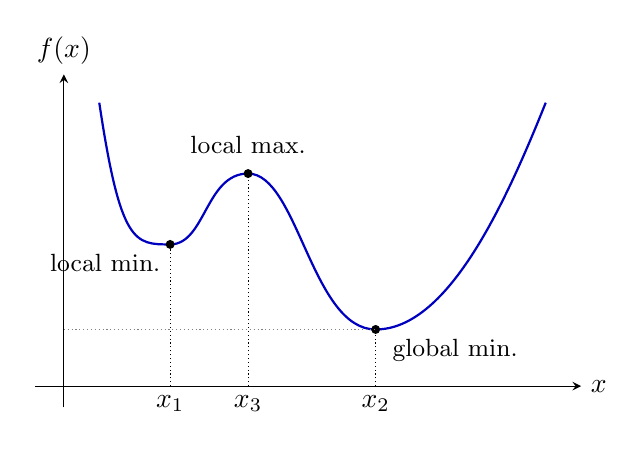
\begin{tikzpicture}[scale=0.9, >=stealth]
		\draw[->] (-0.4,0) -- (7.3,0) node[right] {$x$};
		\draw[->] (0,-0.3) -- (0,4.4) node[above] {$f(x)$};
		\draw[thick,blue!75!black]
		(0.5,4) .. controls (0.8,2) and (1,2) .. (1.5,2)
		.. controls (2,2) and (2,3) .. (2.6,3)
		.. controls (3.3,3) and (3.5,0.8) .. (4.4,0.8)
		.. controls (5.4,0.8) and (6.2,2.5) .. (6.8,4);
		\foreach \x/\y/\lab in {1.5/2/x_1,2.6/3/x_3,4.4/0.8/x_2} {
				\draw[densely dotted] (\x,0) -- (\x,\y);
				\fill (\x,\y) circle (1.8pt);
				\node[below] at (\x,0) {$\lab$};
			}
		\draw[densely dotted,gray] (0,0.8) -- (4.4,0.8);
		\node[below left] at (1.5,2) {\small local min.};
		\node[above] at (2.6,3.15) {\small local max.};
		\node[below right] at (4.5,0.8) {\small global min.};
	\end{tikzpicture}
\end{center}
Every global minimiser is a local minimiser, but the converse need not hold. Knowing the behaviour near $x_1$ does not tell us whether a lower valley exists elsewhere. This is why local information alone usually does not establish global optimality. In general, finding global minima is a hard problem.

There may be several local minimisers and several global minimisers. However, if a global minimum is attained, its \emph{value} is unique. Indeed, if $\mathbf{x}_1^*$ and $\mathbf{x}_2^*$ are global minimisers, then
\[
	f(\mathbf{x}_1^*)\leq f(\mathbf{x}_2^*)
	\quad\text{and}\quad
	f(\mathbf{x}_2^*)\leq f(\mathbf{x}_1^*).
\]
Therefore, $f(\mathbf{x}_1^*)=f(\mathbf{x}_2^*)$. The inputs can be different even though their outputs agree.

\begin{center}
	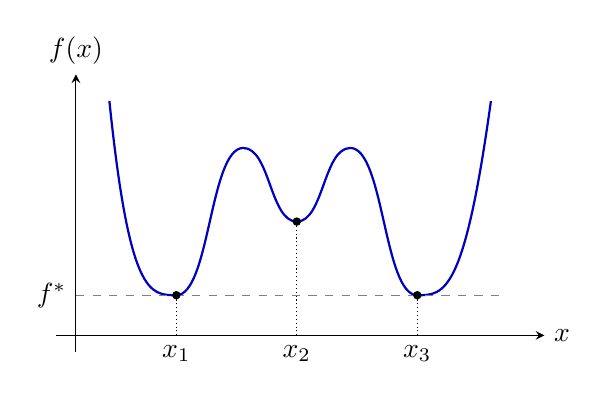
\begin{tikzpicture}[scale=0.85, >=stealth]
		\draw[->] (-0.3,0) -- (7,0) node[right] {$x$};
		\draw[->] (0,-0.25) -- (0,3.9) node[above] {$f(x)$};
		\draw[thick,blue!75!black]
		(0.5,3.5) .. controls (0.8,0.6) and (1.1,0.6) .. (1.5,0.6)
		.. controls (2,0.6) and (2,2.8) .. (2.5,2.8)
		.. controls (2.9,2.8) and (2.9,1.7) .. (3.3,1.7)
		.. controls (3.7,1.7) and (3.7,2.8) .. (4.1,2.8)
		.. controls (4.6,2.8) and (4.6,0.6) .. (5.1,0.6)
		.. controls (5.5,0.6) and (5.8,0.6) .. (6.2,3.5);
		\draw[dashed,gray] (0,0.6) -- (6.4,0.6);
		\node[left] at (0,0.6) {$f^*$};
		\foreach \x/\y/\lab in {1.5/0.6/x_1,3.3/1.7/x_2,5.1/0.6/x_3} {
				\draw[densely dotted] (\x,0) -- (\x,\y);
				\fill (\x,\y) circle (1.8pt);
				\node[below] at (\x,0) {$\lab$};
			}
	\end{tikzpicture}

	\small Three local minimisers; $x_1$ and $x_3$ share the global minimum $f^*$.
\end{center}

\subsection{The role of the feasible set}

Changing the feasible set can change both the location and the existence of an optimum, even when the objective function stays exactly the same.

\begin{example}[The same function on three feasible sets]
	Consider $f(x)=x^2$ and choose $0<a<b$.
	\begin{enumerate}
		\item If $S=\mathbb{R}$, the global minimiser is $x^*=0$ and the minimum value is $0$. There is no local or global maximum.
		\item If $S=[a,\infty)$, then $0$ is infeasible. Since $x^2$ is strictly increasing for $x>0$, the global minimiser is $a$ and the minimum value is $a^2$. There is still no global maximum.
		\item If $S=[a,b]$, the global minimiser is $a$, with value $a^2$, and the global maximiser is $b$, with value $b^2$.
	\end{enumerate}
\end{example}

\begin{center}
	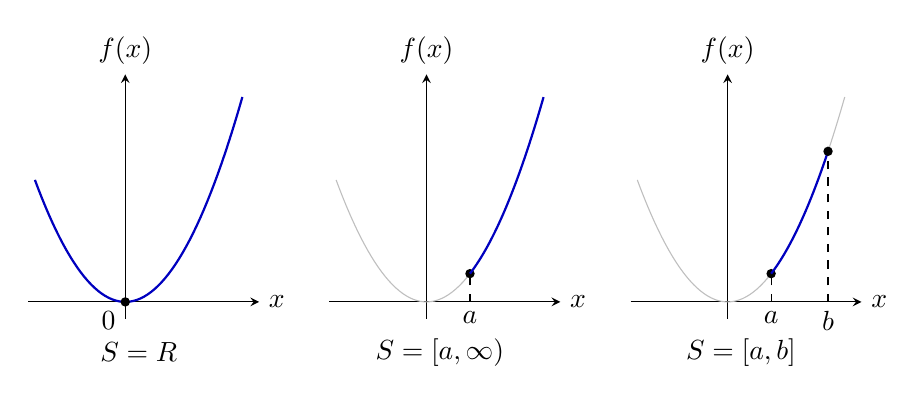
\begin{tikzpicture}[scale=0.85, >=stealth]
		\foreach \shift/\case in {0/1,4.5/2,9/3} {
				\begin{scope}[xshift=\shift cm]
					\draw[->] (-1.45,0) -- (2,0) node[right] {$x$};
					\draw[->] (0,-0.25) -- (0,3.4) node[above] {$f(x)$};
					\draw[gray!50,domain=-1.35:1.75,samples=60]
					plot (\x,{\x*\x});
					\ifnum\case=1
						\draw[thick,blue!75!black,domain=-1.35:1.75,samples=60]
						plot (\x,{\x*\x});
						\fill (0,0) circle (2pt);
						\node[below left] at (0,0) {$0$};
						\node at (0.2,-0.75) {$S=\mathbb{R}$};
					\else
						\draw[dashed] (0.65,0) -- (0.65,0.4225);
						\fill (0.65,0.4225) circle (2pt);
						\node[below] at (0.65,0) {$a$};
						\ifnum\case=2
							\draw[thick,blue!75!black,domain=0.65:1.75,samples=60]
							plot (\x,{\x*\x});
							\node at (0.2,-0.75) {$S=[a,\infty)$};
								\else
								\draw[thick,blue!75!black,domain=0.65:1.5,samples=60]
								plot (\x,{\x*\x});
								\draw[dashed] (1.5,0) -- (1.5,2.25);
								\fill (1.5,2.25) circle (2pt);
								\node[below] at (1.5,0) {$b$};
								\node at (0.2,-0.75) {$S=[a,b]$};
						\fi
					\fi
				\end{scope}
			}
	\end{tikzpicture}

	\small The blue portions correspond to feasible inputs; $0<a<b$.
\end{center}

In the terminology used in class, a \emph{natural extremum} comes from the behaviour of the function itself, without an added restriction on its domain. An \emph{induced extremum} arises because a constraint removes inputs that would otherwise prevent that point from being an extremum.

For $f(x)=x^2$, the minimum at $0$ over $\mathbb{R}$ is natural. The minimum at $a>0$ over $[a,\infty)$ is induced by the constraint. Over $[a,b]$, with $0<a<b$, both the minimum at $a$ and the maximum at $b$ are induced. They are also local extrema relative to the feasible set.

If the feasible interval includes $0$, the natural minimiser remains feasible.

\begin{definition}[Constrained and unconstrained optimisation]
	If we restrict the allowed inputs beyond the domain of the function, we have a \emph{constrained optimisation problem}. If $S=\mathrm{Dom}\,f$, so that no additional restriction is imposed, we have an \emph{unconstrained optimisation problem}.
\end{definition}

For most of the initial part of this course, we will study unconstrained problems. Constraints will be considered later. The derivative tests below concern interior points where movement in both directions is possible.

\section{Unconstrained optimisation of smooth single-variable functions}

We now consider functions $f:\mathbb{R}\to\mathbb{R}$, or more generally $f:I\to\mathbb{R}$ on an open interval $I$, with no additional constraints.

\begin{definition}[Smooth function]
	A function on an open interval is called \emph{smooth} if it has continuous derivatives of every order; that is, it can be differentiated infinitely many times.
\end{definition}

\begin{example}
	Polynomials, $e^x$, $\sin x$ and $\cos x$ are smooth on $\mathbb{R}$. A polynomial is still infinitely differentiable: after sufficiently many derivatives we obtain the zero function, which can be differentiated again. Functions such as $1/x$ and $\tan x$ are smooth on open intervals within their domains, but are not defined on all of $\mathbb{R}$.
\end{example}
\begin{nonexample}
	The function $|x|$ is not differentiable at $0$.
\end{nonexample}

\subsection{First and second derivative tests}

\begin{theorem}[First-order necessary condition]
	Let $x^*$ be an interior point of the domain of $f$, and suppose $f$ is differentiable at $x^*$. If $x^*$ is a local minimiser or a local maximiser, then
	\begin{equation}
		f'(x^*)=0.
		\label{eq:lec04-stationary}
	\end{equation}
\end{theorem}

For the smooth functions considered here, we find the \emph{critical points} by solving $f'(x)=0$. Each is only a candidate for a local optimiser and must still be checked.

\begin{theorem}[Second derivative test]
	Suppose $f$ has continuous first and second derivatives near an interior point $x^*$, and $f'(x^*)=0$.
	\begin{enumerate}
		\item If $f''(x^*)>0$, then $x^*$ is a local minimiser.
		\item If $f''(x^*)<0$, then $x^*$ is a local maximiser.
		\item If $f''(x^*)=0$, this test is inconclusive.
	\end{enumerate}
\end{theorem}

\begin{example}[The test works for $x^2$]
	Let $f(x)=x^2$. Then
	\[
		f'(x)=2x=0\iff x^*=0,
		\qquad f''(x)=2,
		\qquad f''(0)=2>0.
	\]
	Thus, $0$ is a local minimiser. In fact, $x^2\geq0=f(0)$ for all $x\in\mathbb{R}$, so $0$ is also the unique global minimiser.
\end{example}

\newpage
\begin{example}[The test is inconclusive for $x^4$]
	Let $f(x)=x^4$. Then
	\[
		f'(x)=4x^3=0\iff x^*=0,
		\qquad f''(x)=12x^2,
		\qquad f''(0)=0.
	\]
	The second derivative test gives no conclusion. Nevertheless, $x^4>0=f(0)$ for every $x\neq0$, so $0$ is the unique global minimiser. A zero second derivative does not mean there is no extremum.
\end{example}

\begin{example}[Zero first derivative does not guarantee an extremum]
	Let $f(x)=x^3$. Then
	\[
		f'(x)=3x^2=0\iff x^*=0,
		\qquad f''(x)=6x,
		\qquad f''(0)=0.
	\]
	For every $h>0$, we have $f(-h)<f(0)<f(h)$. Thus, $0$ is neither a local minimiser nor a local maximiser. The same pair of values $f'(0)=f''(0)=0$ occurs for $x^4$, but the behaviour is different.
\end{example}

\begin{center}
	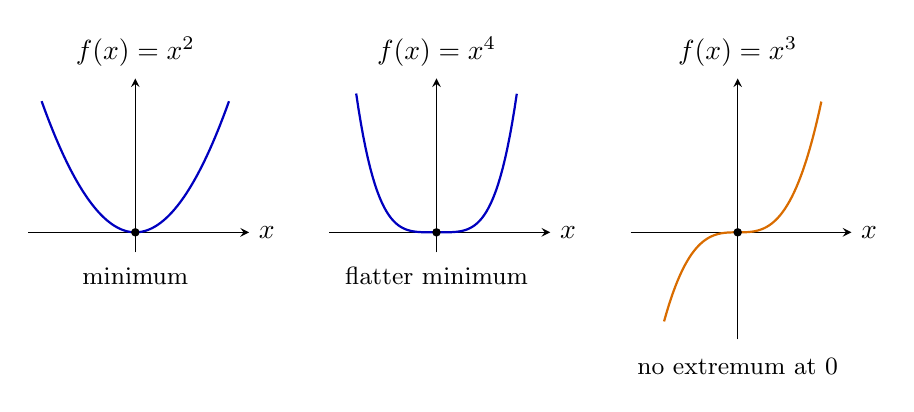
\begin{tikzpicture}[scale=0.85, >=stealth]
		\begin{scope}
			\draw[->] (-1.6,0) -- (1.7,0) node[right] {$x$};
			\draw[->] (0,-0.3) -- (0,2.3);
			\draw[thick,blue!75!black,domain=-1.4:1.4,samples=70]
			plot (\x,{\x*\x});
			\fill (0,0) circle (1.8pt);
			\node at (0,2.7) {$f(x)=x^2$};
			\node at (0,-0.65) {\small minimum};
		\end{scope}
		\begin{scope}[xshift=4.5cm]
			\draw[->] (-1.6,0) -- (1.7,0) node[right] {$x$};
			\draw[->] (0,-0.3) -- (0,2.3);
			\draw[thick,blue!75!black,domain=-1.2:1.2,samples=70]
			plot (\x,{\x*\x*\x*\x});
			\fill (0,0) circle (1.8pt);
			\node at (0,2.7) {$f(x)=x^4$};
			\node at (0,-0.65) {\small flatter minimum};
		\end{scope}
		\begin{scope}[xshift=9cm]
			\draw[->] (-1.6,0) -- (1.7,0) node[right] {$x$};
			\draw[->] (0,-1.6) -- (0,2.3);
			\draw[thick,orange!85!black,domain=-1.1:1.25,samples=70]
			plot (\x,{\x*\x*\x});
			\fill (0,0) circle (1.8pt);
			\node at (0,2.7) {$f(x)=x^3$};
			\node at (0,-2) {\small no extremum at $0$};
		\end{scope}
	\end{tikzpicture}
\end{center}

\subsection{Taylor expansion and higher derivative test}
To understand these tests, compare the value at $x^*$ with the value at a nearby point $x^*+h$. A positive $h$ moves to the right; a negative $h$ moves to the left. At a local minimum, we require
\begin{equation}
	f(x^*+h)-f(x^*)\geq0
	\qquad\text{for all sufficiently small }|h|.
	\label{eq:lec04-local-difference}
\end{equation}
At a local maximum, the difference is nonpositive.

\begin{center}
	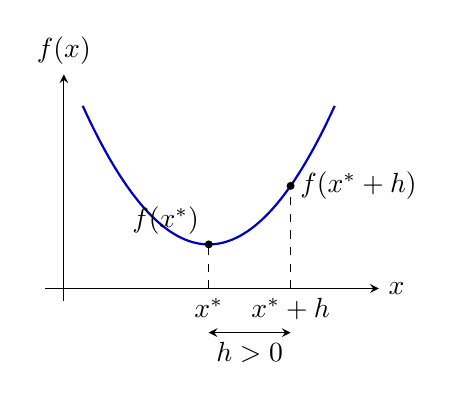
\begin{tikzpicture}[scale=0.8, >=stealth]
		\draw[->] (-2.6,0) -- (2.7,0) node[right] {$x$};
		\draw[->] (-2.3,-0.2) -- (-2.3,3.4) node[above] {$f(x)$};
		\draw[thick,blue!75!black,domain=-2:2,samples=70]
		plot (\x,{0.55*\x*\x+0.7});
		\draw[dashed] (0,0) -- (0,0.7);
		\draw[dashed] (1.3,0) -- (1.3,1.6295);
		\fill (0,0.7) circle (1.8pt);
		\fill (1.3,1.6295) circle (1.8pt);
		\node[above left] at (0,0.7) {$f(x^*)$};
		\node[right] at (1.3,1.6295) {$f(x^*+h)$};
		\node[below] at (0,0) {$x^*$};
		\node[below] at (1.3,0) {$x^*+h$};
		\draw[<->] (0,-0.7) -- (1.3,-0.7) node[midway,below] {$h>0$};
	\end{tikzpicture}
\end{center}

A function is \emph{analytic} near a point if it agrees with its Taylor series there. Smoothness alone does not guarantee this. As in the lecture, assume here that $f$ is analytic near $x^*$, so that we can write
\begin{equation}
	f(x^*+h)=f(x^*)+h f'(x^*)
	+\frac{h^2}{2!}f''(x^*)
	+\frac{h^3}{3!}f^{(3)}(x^*)+\cdots.
	\label{eq:lec04-taylor-series}
\end{equation}
Here, $f^{(k)}(x^*)$ denotes the $k$th derivative evaluated at $x^*$. Each of these evaluated derivatives is a fixed number; $h$ is the quantity that varies.

\textbf{Why must the first derivative vanish?}
Subtracting $f(x^*)$ from the Taylor expansion gives
\[
	f(x^*+h)-f(x^*)
	=h f'(x^*)+\frac{h^2}{2!}f''(x^*)+\cdots.
\]
For sufficiently small $|h|$, the first nonzero term determines the sign of this difference. If $f'(x^*)\neq0$, the leading term $h f'(x^*)$ changes sign when we move from the right of $x^*$ to the left. The difference then cannot stay nonnegative on both sides, as a local minimum requires. It cannot stay nonpositive on both sides either. Therefore, at a local optimiser we must have $f'(x^*)=0$.

\textbf{Why does the second derivative classify the point?}
When $f'(x^*)=0$, the expansion starts with
\begin{equation}
	f(x^*+h)-f(x^*)
	=\frac{h^2}{2!}f''(x^*)+\frac{h^3}{3!}f^{(3)}(x^*)+\cdots.
	\label{eq:lec04-second-order}
\end{equation}
If $f''(x^*)\neq0$, the quadratic term determines the sign for sufficiently small nonzero $h$. Since $h^2$ is positive on both sides, $f''(x^*)>0$ makes the nearby values larger, giving a local minimum. Similarly, $f''(x^*)<0$ makes them smaller, giving a local maximum.

\textbf{What if the second derivative also vanishes?}
If $f'(x^*)=f''(x^*)=0$, we look at the next terms:
\begin{equation}
	f(x^*+h)-f(x^*)
	=\frac{h^3}{3!}f^{(3)}(x^*)
	+\frac{h^4}{4!}f^{(4)}(x^*)+\cdots.
	\label{eq:lec04-third-fourth-order}
\end{equation}
If $f^{(3)}(x^*)\neq0$, the leading cubic term changes sign across $x^*$, so there is no local minimum or maximum. If $f^{(3)}(x^*)=0$ but $f^{(4)}(x^*)\neq0$, the fourth-order term comes first. Since $h^4>0$ for $h\neq0$, a positive $f^{(4)}(x^*)$ gives a local minimum and a negative value gives a local maximum. If this derivative also vanishes, we look at the next order. The rule below applies once a first nonzero derivative is found.

\begin{theorem}[First nonzero derivative test]
	Let $f$ be analytic near an interior point $x^*$, as assumed in the Taylor argument above. Suppose, for some integer $m\geq1$,
	\begin{equation}
		f^{(k)}(x^*)=0\quad(1\leq k<m),
		\qquad f^{(m)}(x^*)\neq0.
		\label{eq:lec04-first-nonzero}
	\end{equation}
	Then:
	\begin{enumerate}
		\item If $m$ is odd, $x^*$ is neither a local minimiser nor a local maximiser.
		\item If $m$ is even and $f^{(m)}(x^*)>0$, then $x^*$ is a local minimiser.
		\item If $m$ is even and $f^{(m)}(x^*)<0$, then $x^*$ is a local maximiser.
	\end{enumerate}
\end{theorem}
\begin{proof}
	In the Taylor argument above, the terms before order $m$ vanish. Thus, the first nonzero term in $f(x^*+h)-f(x^*)$ is
	\[
		\frac{h^m}{m!}f^{(m)}(x^*).
	\]
	For sufficiently small nonzero $h$, this term determines the sign. If $m$ is odd, $h^m$ changes sign between the two sides, so there can be no local minimum or maximum. If $m$ is even, $h^m$ is positive on both sides. The sign is then the sign of $f^{(m)}(x^*)$: positive gives a local minimum, and negative gives a local maximum.
\end{proof}

Once the first nonzero derivative is found, later derivatives do not affect this classification; they need not vanish. In particular, the test does not require every odd-order derivative to be zero at a local optimum.

Returning to $f(x)=x^4$, we have $f^{(3)}(x)=24x$ and $f^{(4)}(x)=24$. At $0$, the first nonzero evaluated derivative has even order $4$ and is positive, confirming a local minimum. For $f(x)=x^3$, $f^{(3)}(0)=6\neq0$ has odd order, so $0$ is neither a local minimum nor a local maximum.

\begin{remark}[The test need not finish for every smooth function]
	Being smooth does not guarantee that a first nonzero derivative will be found. For example, the smooth function
	\[
		q(x)=\begin{cases}
			e^{-1/x^2}, & x\neq0, \\
			0,          & x=0
		\end{cases}
	\]
	has $q^{(k)}(0)=0$ for every $k\geq1$. Nevertheless, $0$ is a global minimiser, since $q(0)=0$ and $q(x)>0$ for $x\neq0$. Thus, if all evaluated derivatives vanish, the higher derivative test gives no conclusion; we need another argument.
\end{remark}

\begin{example}[Cubic function]
	Find the local minima and maxima of
	\begin{equation}
		f(x)=x^3-6x^2+11x-6,
		\qquad x\in\mathbb{R}.
		\label{eq:lec04-cubic}
	\end{equation}
\end{example}

\textbf{Solution.}
First, note that
\[
	f(x)=(x-1)(x-2)(x-3).
\]
Thus, the graph crosses the $x$-axis at $1$, $2$ and $3$. To locate the possible local optimisers, we solve $f'(x)=0$.

\textbf{Step 1: Find the candidates.}
Differentiating gives
\[
	f'(x)=3x^2-12x+11.
\]
Hence,
\begin{align}
	3x^2-12x+11 & =0,\notag                            \\
	x           & =\frac{12\pm\sqrt{144-132}}{6}\notag \\
	            & =\frac{12\pm\sqrt{12}}{6}
	=2\pm\frac{\sqrt{3}}{3}
	=2\pm\frac{1}{\sqrt{3}}.
	\label{eq:lec04-cubic-stationary}
\end{align}
Following the board notation, let
\[
	x_1^*=2+\frac{1}{\sqrt{3}},
	\qquad x_2^*=2-\frac{1}{\sqrt{3}}.
\]
Notice that $x_2^*<x_1^*$.

\textbf{Step 2: Classify each candidate separately.}
We have $f''(x)=6x-12$. Therefore,
\begin{align*}
	f''(x_1^*) & =6\left(2+\frac{1}{\sqrt{3}}\right)-12
	=\frac{6}{\sqrt{3}}=2\sqrt{3}>0,                    \\
	f''(x_2^*) & =6\left(2-\frac{1}{\sqrt{3}}\right)-12
	=-\frac{6}{\sqrt{3}}=-2\sqrt{3}<0.
\end{align*}
Thus, $x_1^*$ is a local minimiser and $x_2^*$ is a local maximiser. Both classifications stop at the second derivative because it is already nonzero at each point.

\textbf{Step 3: Find the corresponding optimum values.}
Set $t=x-2$. Then
\begin{align*}
	f(2+t)
	 & =(2+t)^3-6(2+t)^2+11(2+t)-6              \\
	 & =(8+12t+6t^2+t^3)-(24+24t+6t^2)+22+11t-6 \\
	 & =t^3-t.
\end{align*}
Consequently,
\begin{align*}
	f(x_1^*) & =\left(\frac{1}{\sqrt{3}}\right)^3
	-\frac{1}{\sqrt{3}}
	=-\frac{2}{3\sqrt{3}},                         \\
	f(x_2^*) & =\left(-\frac{1}{\sqrt{3}}\right)^3
	+\frac{1}{\sqrt{3}}
	=\frac{2}{3\sqrt{3}}.
\end{align*}
These are the local minimum and local maximum \emph{values}, respectively.

\begin{center}
	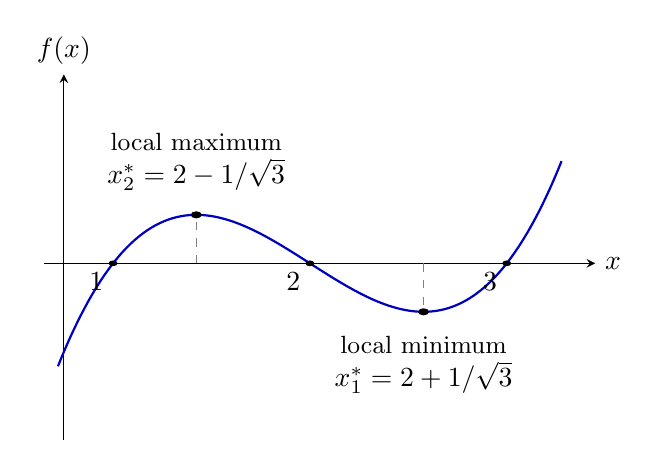
\begin{tikzpicture}[xscale=2.5,yscale=1.6, >=stealth]
		\draw[->] (0.65,0) -- (3.45,0) node[right] {$x$};
		\draw[->] (0.75,-1.4) -- (0.75,1.5) node[above] {$f(x)$};
		\draw[thick,blue!75!black,domain=0.72:3.28,samples=120]
		plot (\x,{(\x-1)*(\x-2)*(\x-3)});
		\foreach \x in {1,2,3} {
				\fill (\x,0) circle (0.65pt);
				\node[below left] at (\x,0) {$\x$};
			}
		\draw[dashed,gray] (1.42265,0) -- (1.42265,0.38490);
		\draw[dashed,gray] (2.57735,0) -- (2.57735,-0.38490);
		\fill (1.42265,0.38490) circle (0.8pt);
		\fill (2.57735,-0.38490) circle (0.8pt);
		\node[above,align=center] at (1.42265,0.5)
		{\small local maximum\\$x_2^*=2-1/\sqrt{3}$};
		\node[below,align=center] at (2.57735,-0.5)
		{\small local minimum\\$x_1^*=2+1/\sqrt{3}$};
	\end{tikzpicture}
\end{center}

\textbf{Step 4: Check whether the extrema are global.}
Since the leading term is $x^3$,
\[
	\lim_{x\to\infty}f(x)=\infty,
	\qquad \lim_{x\to-\infty}f(x)=-\infty.
\]
Thus, on $S=\mathbb{R}$ the function has neither a global minimiser nor a global maximiser. The two points found above give only local extrema. As a check, $f'(x)=3(x-x_2^*)(x-x_1^*)$ is positive before $x_2^*$, negative between $x_2^*$ and $x_1^*$, and positive after $x_1^*$. The graph therefore increases, decreases, and then increases again, consistent with the classifications above.

Different candidate points may require different numbers of derivatives. At each candidate, we stop at the first nonzero \emph{evaluated} derivative; the derivative function need not be identically zero.

Finally, interior differentiability is essential for the necessary condition $f'(x^*)=0$. For example, $|x|$ has a minimum at $0$, where the derivative does not exist. Similarly, $x^2$ on $[a,\infty)$ with $a>0$ has its minimum at $a$, although $f'(a)=2a\neq0$. At a constrained boundary, we cannot move in both directions while remaining feasible, so the argument for \eqref{eq:lec04-stationary} does not apply. We will study the appropriate conditions for constrained optimisation later.


\lecture_date{27/10/2026}
\chapter{Lecture 05}

\section{Unconstrained optimisation of smooth single-variable functions---continued}
\subsection{Taylor expansion and higher derivative test---continued}

Based on the theorems developed in the last lecture, we will workout on another example.

\begin{exercise}
	Consider the function $f:\mathbb{R}\to\mathbb{R}$ given by
	\begin{equation}
		f(x)=(5x^5+3x^3)e^x.
		\label{eq:lecture05-function}
	\end{equation}
	Find its local maximisers/minimizers, and their local maxima/minima.
\end{exercise}
\begin{answer}
	Applying the product rule to \autoref{eq:lecture05-function}, we get
	\begin{align}
		f'(x)
		 & = (25x^4+9x^2)e^x+(5x^5+3x^3)e^x \notag \\
		 & = x^2e^x(5x^3+25x^2+3x+9).
		\label{eq:lecture05-first-derivative}
	\end{align}
	As $e^x>0$ for every $x\in\mathbb{R}$, by \autoref{thm:first-order-necessary-condition}, potential local minimizers (aka. critical points) are determined by the equation
	\begin{equation}
		x^2(5x^3+25x^2+3x+9)=0.
		\label{eq:lecture05-stationary}
	\end{equation}
	Thus, $x=0$ is a critical point. The remaining critical points satisfy
	\begin{equation}
		5x^3+25x^2+3x+9=0.
		\label{eq:lecture05-cubic}
	\end{equation}
	The cubic polynomial in \autoref{eq:lecture05-cubic} has exactly one real root. Numerically, this root is
	\[
		\alpha\approx -4.952238165.
	\]
	Hence, the function has two distinct critical points, namely $x=\alpha$ and $x=0$.

	To classify these points, we compute the second derivative:
	\begin{equation}
		f''(x)
		=xe^x(5x^4+50x^3+103x^2+18x+18).
		\label{eq:lecture05-second-derivative}
	\end{equation}
	At $x=\alpha$,
	\[
		f''(\alpha)\approx21.3643>0.
	\]
	Hence, by \autoref{thm:second-derivative-test}, $\alpha$ is a local minimizer. The corresponding local minimum is
	\[
		f(\alpha)\approx-107.831366.
	\]

	At $x=0$,
	\[
		f'(0)=0,\qquad f''(0)=0.
	\]
	Thus, the second-order test is inconclusive. We therefore apply \autoref{thm:first-nonzero-derivative-test}:

	Differentiating \autoref{eq:lecture05-second-derivative},
	we get
	\begin{equation}
		f'''(x) = e^x(5x^5+75x^4+303x^3 +327x^2+72x+18).
		\label{eq:taylor-expansion-and-higher-derivative-test-continued-1}
	\end{equation}
	In particular,
	\[
		f'''(0)=18\neq0.
	\]
	Therefore,
	\[
		f'(0)=f''(0)=0,
		\qquad f'''(0)\neq0.
	\]
	So first nonzero derivative at $x=0$ is of order $m=3$. Since $m$ is odd, $x=0$ is neither a local minimiser nor a local maximiser.

	We conclude that there is no local maxima of \( f \), and it a has local minimizer at \( x^\ast \approx-4.952238165 \) and corresponding minimum is \( f(x^\ast) \approx-107.831366 \).
\end{answer}


\printbibliography[title=References]

\end{document}
